\section{Theoretical Analysis} \label{section:theo}


\par In this section, a theoretical analysis of the circuit shown in section \ref{introduction} was conducted. 

\subsection{Description and Important Mathematical considerations}


A theoretical approach of the circuit shown in section 1 was conducted. In fact the Op-Amp used was considered ideal, which means that the internal impedance between v+ and v- is infinite and that there is no current flowing through it (v+ = v-). Hence, a band pass filter was built by connecting a capacitor (C1) in series with the input voltage, which will function as a high pass filter. On top of that, in the final stage of the circuit, another capacitor (C2) was connected in parallel with the output voltage, functioning as a low pass filter. All in all, this circuit consists of a high pass filter, a signal amplifier and a low pass filter in series. 


The transfer function of the circuit was determined. Accordingly to what was learned in lectures and in the presential laboratory class, we reached the following conclusion:

\begin{equation}
T(s)= \frac{Vout(s)}{Vin(s)}=1+\frac{Zout(s)}{Zin(s)} = \frac{R1*C1*s}{1+R1*C1*s}*(1+\frac{R3}{R4})*\frac{1}{1+R2*C2*s}
\end{equation}

In fact, the gain is given by the product of these 3 expressions ($A_{V}$, $A_{H}$, $A_{L}$), where $A_{V}$ is the gain that results from the OP-AMP (signal amplifier), $A_{H}$ and $A_{L}$ are the gains that correspond to the high pass and low pass filters, respectively.

\begin{equation}
A_{V}=  1+\frac{R3}{R4}
\end{equation}

\begin{equation}
A_{L}=  \frac{1}{1+R2*C2*s}
\end{equation}

\begin{equation}
A_{H}=  \frac{R1*C1*s}{1+R1*C1*s}
\end{equation}


Using the previous calculations we were able to determine the gain , which is shown below.

\begin{table}[ht]
  \centering
  \begin{tabular}{|l|r|}
    \hline    
    {\bf Name} & {\bf Value} \\ \hline
    \input{../mat/wo_freq_gain_tab}
  \end{tabular}
  \caption{Central Frequency(Hz) and Respective Gain(dB).}
\end{table}

So that it can be better understood, and as it was requested, the gain frequency response was ploted. As one may observe, both low and high frequencies have a reduced gain. On the contrary, the frequencies in the central frequency (near to 1KHz) have a maximum gain associated. As it was expected for a band pass filter. This is due to the fact that, in the first stage, the high pass filter blocks the low frequencies (for low frequencies, the impedance goes to infinity and the capacitor is basically an open circuit)  and, in the final stage the low pass filter does not allow the high frequencies to pass (for high impedances, the impedance goes to 0 and the capacitor is basically a short circuit). In fact, at the central frequency, both $A_{L}$ and $A_{H}$ are approximately 1. Hence $A_{V}$ is the one that should be maximized.

\newpage

\begin{figure}[h] \centering
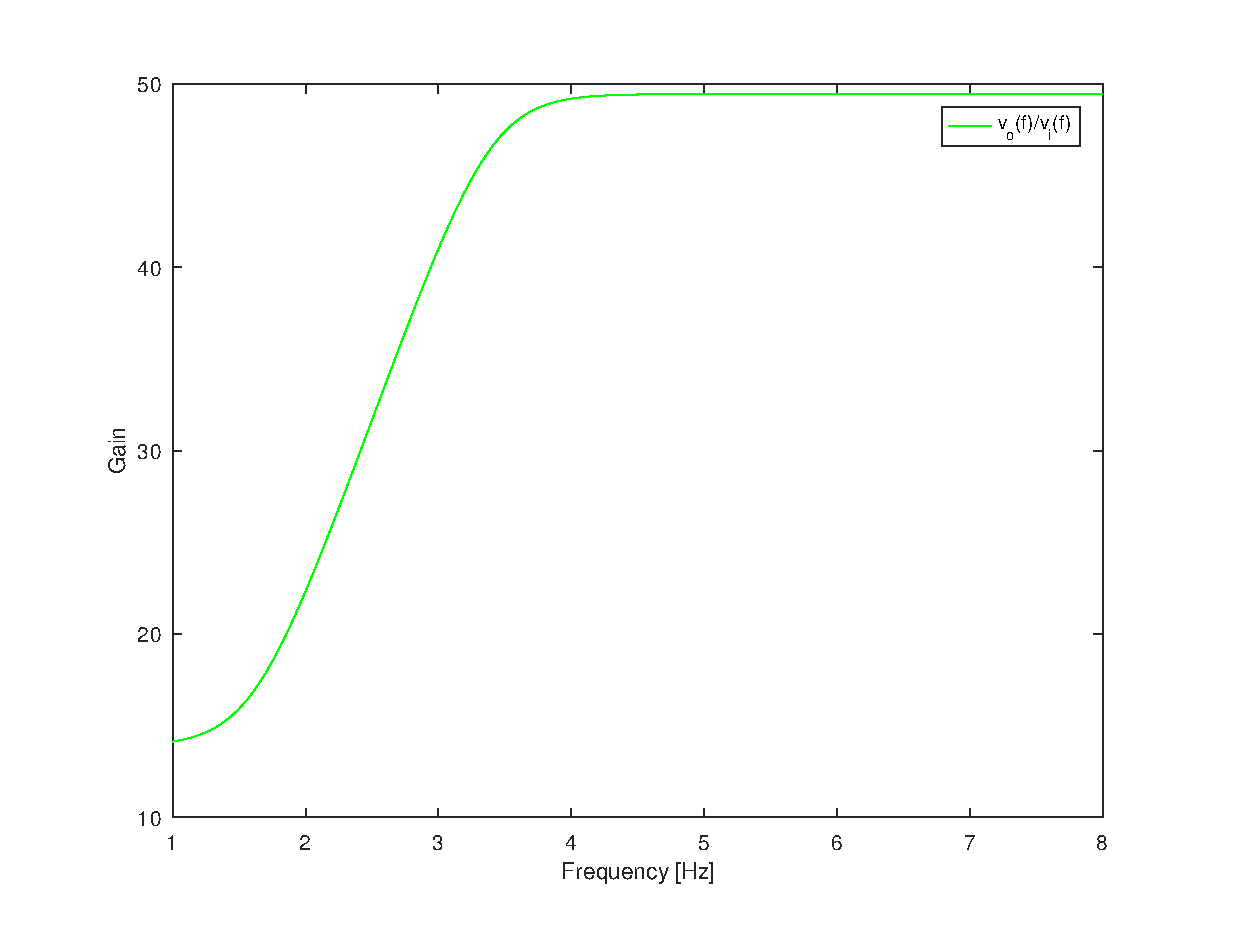
\includegraphics[width=0.45\linewidth]{theo.eps}
\caption{Phase Frequency Response.}
\label{sh}
\end{figure}

\begin{figure}[h] \centering
\includegraphics[width=0.45\linewidth]{theo_phase.eps}
\caption{Gain Frequency Response.}
\label{sh2}
\end{figure}


We also computed the low cutoff frequency and the high cut off frequency in octave. The central frequency was also calculated. The equations and the results computed are the following:


\begin{equation}
\omega_{L}= \frac{1}{R1*C1}
\end{equation}

\begin{equation}
\omega_{H}= \frac{1}{R2*C2}
\end{equation}

\begin{equation}
\omega_{0}= \sqrt{\omega_{L} * \omega_{H}}
\end{equation}



\begin{table}[ht]
  \centering
  \begin{tabular}{|l|r|}
    \hline    
    {\bf Name} & {\bf Value} \\ \hline
    \input{../mat/band_pass_freq_tab}
  \end{tabular}
  \caption{Low cut-off frequency, High cut-off frequency, Central Frequency.}
\end{table}


As requested, the input and output impedances were also calculated as follows:

\begin{equation}
Z_{in}= R1+ \frac{1}{j*\omega_{0}*C1} 
\end{equation}

\begin{equation}
Z_{out}= \frac{R2}{j*\omega_{0}*C2*(R2+\frac{1}{j*\omega_{0}*C2})} 
\end{equation}

The results of the input and output impedances are presented in the table below. The central frequency previouly calculated was considered.

\begin{table}[ht]
  \centering
  \begin{tabular}{|l|r|}
    \hline    
    {\bf Name} & {\bf Value} \\ \hline
    \input{../mat/impedances_tab}
  \end{tabular}
  \caption{Input and output Impedences [Ohm]}
  \label{tab:2}
\end{table}


The figure of merit was also computed, following the expression presented in section \ref{introduction}.

\begin{table}[ht]
  \centering
  \begin{tabular}{|l|r|}
    \hline    
    {\bf Name} & {\bf Value} \\ \hline
    \input{../mat/Cost_Merit_tab}
  \end{tabular}
  \caption{Cost and Merit.}
\end{table}



